%% This file is a portion of the source for Revised Edition 1.1 of
%% Operating Systems and Middleware: Supporting Controlled
%% Interaction, Copyright 2011 by Max Hailperin.  This work is
%% licensed under the Creative Commons Attribution-ShareAlike 3.0
%% Unported License. To view a copy of this license, visit
%% http://creativecommons.org/licenses/by-sa/3.0/ or send a letter to
%% Creative Commons, 171 Second Street, Suite 300, San Francisco,
%% California, 94105, USA.
\chapter{Networking}
\label{networking-chapter}

\section{Introduction}

The overarching theme of this book is how computations interact with
one another with support from operating systems and middleware.  In
Chapter~\ref{persistence-chapter} you saw that computations running at different
times can interact by using persistent storage.  In this chapter,
you will see that computations can be distributed in space as well as
time by sending messages across networks.

Networking is a topic that merits its own courses and textbooks.  My
goal here is to give an overview or review, depending on whether you
have studied the topic before.  I particularly highlight the ways in
which networking ties in with the division of responsibilities
between operating systems, middleware, and application software.
Chapter~\ref{distmid-chapter} goes into more depth on the middleware commonly used to
support distributed applications.

Because black boxes are inimical to education, I
provide more detail about networking than is absolutely
necessary for the development of distributed systems.  However, my
objective is not to make you a network engineer, capable of monitoring
congestion and configuring routers, or even to give you a start
towards that goal.  (Though if you do pursue that goal, my overview
of networking should not hurt you.)  Instead, I am trying to
explain the foundations that underlie distributed systems.  In this
chapter, not only do I spend a lot of time on the foundations, but also some time on
such higher-level structures as the web and distributed file systems.
Chapter~\ref{distmid-chapter} moves completely away from networking per se and into
the middleware most commonly used to build distributed systems.

\subsection{Networks and Internets}\label{networks-and-internets-section}

Before going any further, I should be clear about the meaning of three
closely related terms: ``a network,'' ``an internet,'' and ``the
Internet.''  I will start by describing what networks and internets
have in common and then describe the essential difference.  Once you
understand the general concept of an internet, I will be able to
define the Internet as one specific internet.

A network is a collection of \vocabs{link}
and \vocabes{switch}; so is an internet.  Links are communication channels, such
as wires, optical fibers, or radio channels.  Switches are devices
that connect links together and forward data between them. Some switches are known by more
specific names; for example, those that connect radio links to wired
links are known as \vocabs{access point}, and those that connect the
constituent networks of an internet are known as \vocabs{router}, as I
will discuss subsequently.

Both networks and internets have computers interfaced to some of the
links, as shown in in Figure~\ref{scan-9-1}, with each
interface identified by an address.
\begin{figure}
\centerline{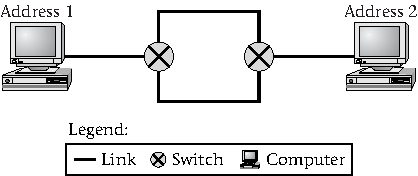
\includegraphics{hail_f0901}}
%\centerline{\def\epsfsize#1#2{0.6#1}\epsfbox{scan-9-1.eps}}
\caption{This network (or internet) contains four links, two switches,
  and two interfaced computers.  Two alternative
  paths connect the two computers.  As described in the text, more
  information would be needed to determine whether this is a picture
  of a single network or an interconnected group of networks, that is, an
  internet.}
\label{scan-9-1}
\end{figure}
Any interfaced computer can
transmit data tagged with a destination address, and under normal
circumstances the data will make its way through the appropriate
links and switches so as to arrive at the specified
destination.  (As a simplification, I will ignore \vocab{multicast},
in which a single message can be delivered to more than one
destination interface.)  A chunk of data tagged with an address is informally called a \vocab{packet}; later I will introduce a variety of more specific terms (\vocab{datagram}, \vocab{segment}, and \vocab{frame}), each of which is synonymous with \vocab{packet} but implies a particular context.

For a single \vocab{network}, as opposed to an internet, the preceding
description is essentially the entire story.  Data injected into the
network is tagged only with the destination address, not with any
information about the route leading to that address.  Even the word
``address'' may be misleading; addresses on a network do not convey
any information about physical location.  If you move a computer
to somewhere else on the same network, it will
still have the same address.

Thus, a packet of data with a network address is not like an envelope
addressed to ``800 W.\ College Ave., St.\ Peter, MN 56082, USA,'' but rather
like one addressed to ``Max Hailperin.''  The network needs to figure
out where I am, as well as what path through the links and
switches leads to that location.  As such, the switches
need to take considerable responsibility.

In part, switches within networks shoulder their
responsibility for delivering data by keeping track of each
interface's last known location.  In part, the switches take the
simpler approach of forwarding data every which way, so that it is
sure to run into the destination interface somewhere.  (However, the
forwarding must not be so comprehensive as to cause data to flow in
cycles.)  Neither approach scales well.  As such, networks are
normally confined to a limited number of interfaces, such as one workgroup within a company.  When the network's scale is small
geographically as well as in number of interfaces, it is called a
\vocab{local area network} (\vocab{LAN}).  Conversely, a \vocab{wide
area network} (\vocab{WAN}) ties together interfaces that are far
apart, though they are generally still few in number, perhaps even
just two.

Multiple networks can be linked together into an \vocab{internet}
by using \vocabs{router}, which are switches that connect to more
than one network, as shown in Figure~\ref{scan-9-2}.
\begin{figure}
\centerline{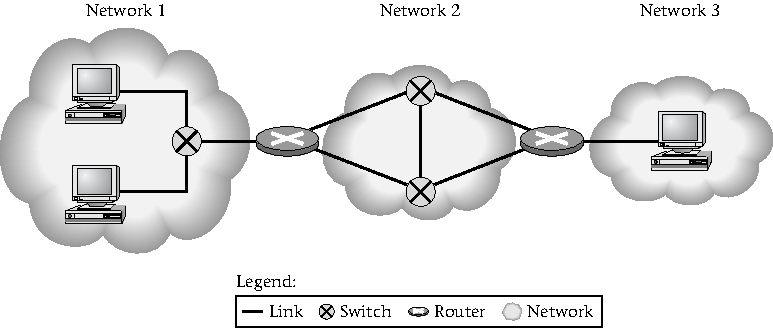
\includegraphics{hail_f0902}}
%\centerline{\def\epsfsize#1#2{0.6#1}\epsfbox{scan-9-2.eps}}
\caption{This internet was formed by connecting three networks.
  Each connection between networks is provided by a router, which is a
  switch interfaced to links belonging to two or more networks.}
\label{scan-9-2}
\end{figure}
In order to distinguish internets from networks, I still
need to explain why linking networks together doesn't just result in a single larger network.

The distinguishing feature of an internet is that the destination
addresses for the the data it conveys are two-part internet addresses,
identifying both the destination network and the specific computer
interface on that network.  Returning to my real-world analogy, a
packet of data with an internet address is like an envelope addressed
to ``Max Hailperin, Gustavus Adolphus College.''  There are people all
over the world (analogous to routers) who could figure out how to
forward the envelope to Gustavus Adolphus College.  Once the envelope
was on my college campus, people (analogous to switches within my local
network) could forward the envelope to me.

Internets work similarly.  Each router figures out what the next
router should be in order to reach the destination network,
independent of the specific computer on that network.  The data is
forwarded from each router to the next using the ordinary mechanisms
of each constituent network, and likewise is forwarded from the last
router to the destination computer using the destination network's
mechanisms.

The two-part structure of internet addresses comes with a cost; when a
computer is moved from one network to another, it
must be assigned a new internet address.  However, in return for this
cost, an internet can scale to a much larger
size than an individual network.  In particular, one internet now
connects such a large fraction of the world's computers that it is
simply known as ``the Internet.''

\subsection{Protocol Layers}\label{protocol-layers-sections}

Network communication is governed by sets of rules, known as
\vocabs{protocol}, which specify the legal actions for each partner in
the dialog at each step along the way.  For example, web browsers
communicate with web servers using HTTP (Hypertext Transfer Protocol),
which specifies the messages the browser and server can legally send
at each step.  In Section~\ref{http-section}, I will show what those
messages actually look like.  For now, however, I will paraphrase the
messages in plain English in order to illustrate the notion of a
protocol.

When a web
browser asks a web server to download a particular web page only if it has
changed since the version the browser has cached, the server may
legitimately respond in several different ways, including:
\begin{itemize}
\item ``It changed; here is the new version.''
\item ``No change, so I won't bother sending the page.''
\item ``I have no clue what page you are talking about.''
\end{itemize}
However, the web server is not allowed to give any of those responses until the
question is asked, and it is also not allowed to give other responses that might be
legal in other circumstances, such as ``I created that new page per
your upload.''  Not surprisingly, HTTP also forbids the web server
from responding with something like
``mailbox full'' that would be appropriate in a different protocol,
the one used to deliver email.

When humans converse, they talk not only about the subject of the
conversation (``We could sure use some rain.'') but also about the
conversation itself (``I didn't catch that, could you say it again?'').
Similarly, computers use not only \foldvocabs{application}{protocol},
like the ones for downloading web pages and sending email messages,
but also \foldvocabs{transport}{protocol}, which control such matters
as retransmitting any portions of the message that get lost.

An application protocol can be viewed as layered on top of a transport
protocol, because the designers of the application protocol take for
granted the services provided by the transport protocol.  With the
most common transport protocol, TCP (Transmission Control Protocol), the
application protocol designers assume the transport protocol will take
care of reliably sending a stream of bytes and having them arrive in
order, without duplication or loss.  All that need concern the
application protocol designer is what the bytes should be to encode
the various messages and responses.  Meanwhile, the transport protocol
designer doesn't worry about what bytes need streaming from one
computer to another, just about the mechanisms for packaging chunks of
bytes with sequence numbers, retransmitting lost chunks, and assembling
the chunks together at the receiving end based on their sequence
numbers.  Thus, the layering of the two protocols results in a
separation of concerns; each protocol can be designed without concern for
the details of the other.

The transport layer is also responsible for allowing each pair of
computers to engage in more than one conversation, a feature known as
\vocab{multiplexing}.  For example, a web browser on my desktop
computer can be requesting web pages from the college's main server at
the same time as my email program is delivering outgoing email to that
same server.  Each transport-layer connection is identified not only
by the internet addresses of the two computers, but also by a
\vocab{port number} on each end, which identifies a specific
communication endpoint.  My web browser connects to one port
number on the server while my email program connects to another.  The
transport-layer software on the receiving computer delivers the data for each port number to the
appropriate application-layer software, that is, it
\vocabes{demultiplex} the arriving data.

The transport protocol can in turn be simplified by assuming that it
has a \foldvocab{network}{protocol} under it, which makes its best
effort to deliver a chunk of data to an internet address.  The
transport protocol may use this service for sending fresh chunks of
application data, handed to it from the application layer, or for
sending retransmissions.  It may also use it for its own internal
purposes, such as sending acknowledgments indicating what data has
been received versus what needs retransmission.  Regardless, from the
perspective of the network protocol, these are all just
packets to deliver.  Meanwhile, from the perspective of the transport
layer, delivery just happens; details like routing need not concern
it.

The network layer is actually something of a misnomer, it that it is
responsible for routing data through an internet.
In fact, the most common network protocol is called the Internet Protocol (IP).
This protocol is used to attempt to deliver data to
any internet address, possibly by way of intermediate routers.
Underneath it are two
more layers, which are genuinely concerned with individual networks:
the link and physical layers.  I'll say more about these layers in
Section~\ref{link-physical-layers-section}.  For now, it suffices to say that these are the
layers implemented by networking hardware, such as Ethernet or
Wi-Fi network cards, for wired or wireless LANs, respectively.

Counting up from the bottom of the stack, the physical, link, network, and
transport layers are frequently referred to as layers 1, 2, 3, and 4.
You might think that the application layer is 5, but in fact there are
two layers I omitted, the session and presentation layers, which are
layers 5 and 6.  Therefore, the application
layer is layer 7.  The only reason you need to know these numbers is
because they frequently show up in discussions of networking devices such
as firewalls.  For example, someone may tell you that their firewall
does ``filtering based on level 7 content.''  What this says is that
the firewall looks at the specific contents of web page requests or email
transmissions.

The listing of seven layers, illustrated in Figure~\ref{scan-9-7}, is
known as the \vocab{OSI (Open Systems Interconnection) reference model}.
\begin{figure}
\centerline{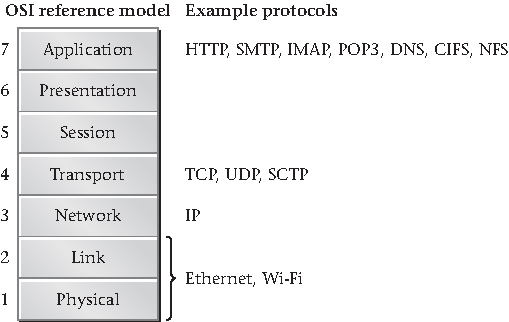
\includegraphics{hail_f0903}}
%\centerline{\def\epsfsize#1#2{0.6#1}\epsfbox{scan-9-7.eps}}
\caption{This diagram of the seven protocol layers in the OSI
  reference model provides
  examples for the layers I discuss.}
\label{scan-9-7}
\end{figure}
I omit layers 5 and 6 from my subsequent discussions because they are
not part of the architecture of the Internet, which
was developed prior to the OSI reference model.  In the Internet
architecture, the application layer takes on the
additional responsibilities, such as character set
encoding and the establishment of network connections, that are
assigned to the presentation and session layers in the OSI reference
model.
I will also largely fold together layers 1
and 2, because the difference doesn't matter unless you are engineering
network hardware.  As such, the bulk of this chapter is divided into
four sections, one each for the application layer~(\ref{application-layer-section}), the transport
layer~(\ref{transport-layer-section}), the network layer~(\ref{network-layer-section}), and the combination of link and
physical layers~(\ref{link-physical-layers-section}).  Those four sections are followed by my usual
section on security~(\ref{network-security-section}), and by
exercises, projects, and notes.

\subsection{The End-to-End Principle}

Traditionally, the Internet has been based on the \vocab{end-to-end
principle}, which states that considerable control and responsibility
should be in the hands of the endpoint computers interfaced to the
Internet's periphery, with the routers and other devices interior to
the Internet providing very simple packet delivery service.  In terms
of the protocol layering, this means that only end computers have
traditionally concerned themselves with the transport and application
protocols.

One virtue of the end-to-end principle is that two users can agree
upon a new application protocol without needing the cooperation of
anyone else.  The ability to try
new application protocols at the grassroots, and see whether they
become popular, was very important in the evolution of the Internet up
through the introduction of the web.

However, the Internet has been progressively moving away from the
end-to-end principle.  I already alluded to one example: firewalls
that filter at the application layer.  I will mention firewalls again
in Section~\ref{fw-ids-section}.  However, there have also been other
non-security-related forces leading away from the end-to-end
principle; I will examine one in Section~\ref{nat-section}.  One upshot
of this is that today it may no longer be possible to just start
using a new application protocol with its associated port number.
Traffic on the new port number might well be blocked as it traverses
the Internet.

This helps explain a popular use of web services, which I explain in
Chapter~\ref{distmid-chapter}.  This form of communications middleware
is often configured to package application programs' messages into
web traffic, in effect layering yet another protocol on top of
the web's application-layer protocol.  This approach helps circumvent obstacles to
new application-layer protocols within the Internet.  For this
chapter, I will stick with the traditional layers, topping out at the
application layer.

\subsection{The Networking Roles of Operating Systems, Middleware, and Application
  Software}

Just as network protocols are layered, so too is the software that
communicates using those protocols.  However, the layering of
networking software does not always correspond directly to the major
divisions that I focus on in this book, between application software,
optional middleware, and an operating system.

The most common division of roles in systems without middleware has
application software responsible for the application-layer protocol,
while the operating system handles everything from transport layer on
down.  That is, the API that operating systems present to application
programs usually corresponds to the services of the transport layer.
This transport-layer API is normally described as providing a
socket abstraction; I will discuss socket APIs in
Section~\ref{socket-APIs}.

In keeping with this division of roles, most application-layer protocols are the
responsibility of application software.  (For example, web browsers and
email programs take responsibility for their respective application
protocols.)  There are a few interesting exceptions, however:
\begin{itemize}
\item
The \vocab{Domain Name System} (\vocab{DNS}) maps names such
as \textit{www.gustavus.edu} into numerical internet addresses such as
138.236.128.22 using an application-layer protocol.  Although
it uses an application-layer protocol, it
plays a critical supporting role for many different applications.  In
most systems, you can best think of the DNS software as a form
of middleware, because it runs outside of the operating system kernel
but supports application software.
\item
Distributed file systems run at the application protocol layer but
need to be visible through the operating system's normal support for
file systems.  Often this means that at least some of the distributed
file system
software is part of the operating system kernel itself, contrary to
the norm for application-layer protocols.
\item
In Chapter~\ref{distmid-chapter}, you will see that many applications are expressed
in terms of more sophisticated communication services than the socket
API.  For example, application programmers may want to send messages that are
queued until received, with the queuing and dequeuing operations
treated as part of atomic transactions.  As another example, application programmers may want to
invoke higher-level operations on objects, rather than just sending
streams of bytes.  In either case, middleware provides the necessary
communication abstractions at the application layer, above the
transport services provided by operating systems.
\end{itemize}

\section{The Application Layer}\label{application-layer-section}

Typical application-layer protocols include HTTP, which is used for
browsing the web, SMTP (Simple Mail Transfer Protocol), which is used
for sending email, POP3 (Post Office Protocol--Version 3), which
is used for retrieving email, and IMAP (Internet Message Access Protocol), which is also used for
accessing email.  Rather than examining each of these, I'll present
HTTP as an example in Section~\ref{http-section}.  Then I'll turn to
some less-typical application protocols that play important roles
behind the scenes: the Domain Name System, which I explain in
Section~\ref{dns-section}, and various distributed file systems, which
I explain in Section~\ref{dfs-section}.

\subsection{The Web as a Typical Example}\label{http-section}

When you use a web browser to view a web page, the browser contacts the web
server using an application-layer protocol known as \vocab{HTTP}
(\vocab{Hypertext Transfer Protocol}).  This protocol has a
request-response form; that is, after the browser connects to the
appropriate port on the server (normally port number 80), it sends a
request and then awaits a response from the server.  Both the request
and the response have the same overall format:
\begin{enumerate}
\item An initial line stating
the general nature of the request or response
\item Any number of header
lines providing more detailed information
\item A blank line to separate the header from the body
\item Any
number of lines of message body
\end{enumerate}
The message body is where the actual web page being downloaded (or
uploaded) appears.  For ordinary web browsing, it is empty in the request and
non-empty in the response.  A common case where a request has a
non-empty body is when you fill in a form and submit it.

To take a concrete example, let's see how you could retrieve my home
page, \textit{http://www.gustavus.edu/+max/}, without the benefit of a web
browser.  You can use the program called \verb|telnet| to connect to the
web server's port 80 using the command
\begin{verbatim}
telnet www.gustavus.edu 80
\end{verbatim}
Then you can type in the following three lines, the last of which is blank:
\begin{verbatim}
GET /+max/ HTTP/1.1
Host: www.gustavus.edu

\end{verbatim}
The first of these is the request line stating that you want to get my
home page using version 1.1 of the protocol.  The second is a header
line, indicating which web host you want to get the page from.  This
is necessary because some web servers have different aliases and may
serve different content depending on which host name you are using.
The blank line indicates that no more header lines are being
specified.

At this point, the server should respond with a large number of lines
of output, of which the first ones will look something like
\begin{verbatim}
HTTP/1.1 200 OK
Date: Sun, 16 Jan 2005 01:18:19 GMT
Server: Apache
Last-Modified: Sun, 16 Jan 2005 01:18:25 GMT
ETag: W/"30ba07-b94-21857f40"
Accept-Ranges: bytes
Content-Length: 2964
Connection: close
Content-Type: text/html; charset=UTF-8

<!DOCTYPE HTML PUBLIC "-//W3C//DTD HTML 4.01 Transitional//EN"
       "http://www.w3.org/TR/html4/loose.dtd">
<html lang="en">
<head>
<title>Max Hailperin's home page</title>
</head>
<body>
<h1>Max Hailperin</h1>
\end{verbatim}
and the last two will be
\begin{verbatim}
</body>
</html>
\end{verbatim}

The first line of the response says that the request was OK and will be
satisfied using HTTP version 1.1.  (The number 200 is a status code,
which indicates that the request was successful.) The server then sends
quite a few header lines; you can probably figure out what several of
them mean.  For example, the Content-Length header indicates that my
home page contained 2964 bytes at the time I tried this example.  The
Content-Type line describes how the web browser should interpret the
message body. In this case, it is a text file written using
\vocab{HTML} (\vocab{HyperText Markup Language}) and with the
character set being an international standard known as UTF-8 (Unicode
Transformation Format 8).   The
boundary between the headers and the message body is formed by the
blank line.  If you are familiar with the syntax of HTML, you can see
that the body is indeed written in HTML.  The HTML format is independent
of the HTTP protocol, which can be used for transferring any kind of
file; the most familiar other formats on the web are those used for
images.

The HTTP standard includes many features beyond those shown in this
one simple example.  To illustrate just one more, consider
sending another request, similar to the first but with one additional
header:
\begin{verbatim}
GET /+max/ HTTP/1.1
Host: www.gustavus.edu
If-none-match: W/"30ba07-b94-21857f40"

\end{verbatim}
This time, the reply from the web server is much shorter:
\begin{verbatim}
HTTP/1.1 304 Not Modified
Date: Sun, 16 Jan 2005 01:19:55 GMT
Server: Apache
Connection: close
ETag: W/"30ba07-b94-21857f40"

\end{verbatim}
This corresponds with the scenario described in
Section~\ref{protocol-layers-sections}.  The browser (or a human using
\verb|telnet| to simulate a browser) is asking ``please send this web page
only if it has changed since the version I previously downloaded.''
The version is identified using the \vocab{ETag} (\foldvocab{entity}{tag}) the server provided when it sent the previous
version.  In this case, the version on the server still is the same
(matches the provided tag), so the server just sends a short reply to
that effect.  A browser could use this to validate continuing to use a
cached copy.

\subsection{The Domain Name System: Application Layer as
  Infrastructure}\label{dns-section}

The network layer takes responsibility for routing a packet of data to
a specified internet address.  However, the internet addresses that it
understands are numbers, encoding the destination network and the
specific interface on that network.  Humans don't generally want to
use these numeric addresses; instead, they prefer to use names such as
\textit{www.gustavus.edu}.  Thus, no matter whether you are using HTTP to
browse the web or SMTP to send email,
you are probably also using an additional application-layer
protocol behind the scenes, to translate names into numerical
addresses.  This protocol is known as the \vocab{Domain
  Name System} (\vocab{DNS}), because the hierarchically structured names such as
\textit{www.gustavus.edu} are known as \foldvocabs{domain}{name}.

The Domain Name System is actually a general facility that allows
machines distributed around the Internet to maintain any arbitrary
mappings of domain names to values, not just mappings of computers'
names to their numerical internet addresses.  However, for the
sake of this overview, I will concentrate on how DNS is used in this
one particularly important context.

The use of domain names to refer to internet addresses is quite
analogous to the use of pathnames to refer to files, a topic I
addressed in Section~\ref{file-linking-section}.  In the following
paragraphs, I will describe four aspects of this analogy.  First, both
kinds of names are hierarchical.  Second, both kinds of names can be
either absolute or relative.  Third, both naming systems allow one
object to directly have multiple names.  And fourth, both naming
systems also allow a name to indirectly refer to whatever some other
name refers to.

A domain name such as \textit{www.gustavus.edu} specifies that
\textit{www} should be found as a subdomain of \textit{gustavus}, which is
in turn a subdomain of \textit{edu}.  Thus, the structure of the name is
similar to a pathname from a POSIX file system, which might be
\verb|edu/gustavus/www| for the file \verb|www| within the
subdirectory \verb|gustavus| of the directory \verb|edu|.  The only
two differences are that the components of a domain name are separated
with dots instead of slashes, and that they are listed from most
specific to least specific, rather than the other way around.

In POSIX pathnames, the difference between \verb|edu/gustavus/www| and
\verb|/edu/gustavus/www| (with an initial slash) is that the former
starts by looking for \verb|edu| in the current working directory,
whereas the latter starts from the root directory of the file system.
These two options are called relative and absolute pathnames.  One
little-known fact about the DNS is that domain names also come in
these two varieties.  The familiar domain name \textit{www.gustavus.edu}
is relative, and so may or may not refer to my college's web server,
depending on the context in which it is used.  If you want to be
absolutely sure what you are talking about, you need to use the
absolute domain name \textit{www.gustavus.edu.}\ complete with the dot on
the end.  On the other hand, only a cruel system administrator would
set up a system where \textit{www.gustavus.edu} was interpreted as
\textit{www.gustavus.edu.horrible.com.} rather than the expected site.
The real reason for relative domain names is to allow shorter names
when referring to computers within your own local domain.

My discussion of file linking in Section~\ref{file-linking-section}
explained that the simplest form of linking is when two names directly
refer to the same file.  Similarly, two domain names can directly
refer to the same internet address.  In the DNS, a domain name can
have multiple kinds of information, or \foldvocabs{resource}{record},
each with an associated type.  The domain name has a directly
specified internet address if it has a resource record of type A.
(The letter A is short for address.)  As an example, the domain names
\textit{gustavus.edu.} and \textit{ns1.gustavus.edu.} both have type A
resource records containing the address 138.236.128.18, so both
of these domain names are referring directly to the same internet
address.

Recall that symbolic links (or soft links) are pathnames that do not
refer directly to a file, but rather indirectly to whatever another
pathname refers to.  Similarly, the DNS supports domain names that are
aliases for other domain names.  As an example, the domain name
\textit{www.gustavus.edu.} currently has no type A resource record.
Instead, it has a type CNAME resource record, showing that it is an
alias for \textit{www.gac.edu.}  Looking this second name up in the DNS,
I find that it too is an alias, with a CNAME record referring to
\textit{charlotte.gac.edu}.  Only this third domain name has the actual
type A record, specifying the internet address 138.236.128.22.
This internet address will be returned by a lookup operation on any of
the three alternative domain names.  The domain name at the end of a
chain of aliases is known as the \foldvocab{canonical}{name},
which explains why the resource record type is called CNAME.

In order to translate a name into an address, an application program
such as a web browser uses a system component known as the \vocab{resolver}.
The resolver communicates using the DNS application-layer protocol
with a name server, which provides the requested information.  In most
systems, the resolver is not part of the operating system kernel.
Instead, it is linked into each application program as part of a
shared library.  From the operating system's perspective, the
application program is engaged in network communication with some
remote system; the fact that the communication constitutes DNS lookups
is invisible.  From the perspective of the application programmer,
however, the resolver is part of the supporting infrastructure, not
something that needs programming.  As such, the resolver constitutes
middleware in the technical sense of that word.  However, it is
conventionally marketed as part of the same product as the operating
system, not as a separate middleware product.

The protocol used between the resolver and name server is a
request-response protocol.  The resolver indicates what information it
is looking for, such as an internet address (type A resource record)
for a particular domain name.  The name server responds with the
requested information, an error report, or a referral to another name
server better able to answer the question.

The details of the DNS protocol are somewhat complicated for three
reasons.  One is that the system is designed to be general, not just
suitable for internet address lookups.  The second is that the system
is designed to reliably serve the entire Internet.  Therefore, it
contains provisions for coordinating multiple name servers, as I
outline in the next paragraph.  The third is that the DNS protocol
does not use ordinary lines of text, unlike the HTTP example I showed
earlier.  Instead, DNS messages are encoded in a compact binary
format.  As such, you cannot experiment with DNS using \verb|telnet|.
Exploration Projects \ref{dns-exploration-dig} and
\ref{dns-exploration-ethereal} suggest some alternate ways you can
experiment with DNS.

No one name server contains all the information for the complete DNS,
nor is any given piece of information stored in only a single
name server, under normal circumstances.  Instead, the information is both partitioned and
replicated, in the following three ways:
\begin{itemize}
\item
The hierarchical tree is divided into zones of control that are stored
independently.  For example, my college maintains the information
about all domain names ending in \textit{gustavus.edu.}\ and
\textit{gac.edu.}\ on name servers we control.  Additional resource
records within the DNS itself indicate where the dividing lines are
between zones.
\item
Authoritative information about names in each zone is stored on multiple
name servers to provide failure tolerance and higher performance.
Secondary servers for the zone periodically check with a master server
for updates.  Resource records within the DNS itself list all the
authoritative name servers for each zone.
\item
Name servers cache individual pieces of information they receive from
other name servers in the course of normal operation.  Thus, when I
repeatedly access \textit{www.nytimes.com.}, I don't have to keep
sending DNS queries all the way to the \textit{New York Times}'s name
server.  Instead, my local name server acquires a non-authoritative copy
of the information, which it can continue using for a specified period
of time before it expires.
\end{itemize}

\subsection{Distributed File Systems: An Application Viewed Through
  Operating Systems}\label{dfs-section}

Using HTTP, you can download a copy of a file from a remote server.
Depending on how the server is configured, you may also be able to
upload the file back to the server after editing it.  Given that the
file I am currently editing (containing this chapter) is stored on a
centralized server, I could be making use of this download-edit-upload
process.  Instead, I am taking advantage of a more convenient,
more subtle, kind of application-layer protocol, a distributed file
system.  In order to edit this chapter, or any other file stored on
the central server, I simply access it by pathname, just the same way
I would access a file on the local disk drive.  Through some
behind-the-scenes magic, certain parts of the file system directory
tree are accessed over the network from the server.  Ordinary
file system operations, such as reading and writing, turn into network
messages using the appropriate application-layer protocol.

Distributed file systems are most commonly used within the boundaries
of a particular organization, unlike the protocols previously
discussed.  Perhaps for this reason, several different distributed
file system protocols have remained viable, rather than a single
standard dominating.  Two of the most popular are \vocab{CIFS}
(\vocab{Common Internet File System}) and \vocab{NFS}
(\vocab{Network File System}).  CIFS has primarily been championed by
Microsoft and is commonly found in organizations with a substantial
number of Microsoft Windows systems.  It frequently is still referred
to by its previous name, the \vocab{SMB} (\vocab{Server Message
Block}) protocol.  (The individual messages sent by CIFS continue to be
called Server Message Blocks.)  NFS was developed by Sun Microsystems
and is primarily used at sites where UNIX and Linux systems dominate.
To confuse nomenclature further, one specific feature of CIFS is
called DFS, for Distributed File System.  I won't discuss that feature
here and will continue to use the the phrase with lower-case letters to
refer to distributed file systems in general.

As I will describe shortly, the designs of CIFS and NFS differ in some
important regards.  However, they also have quite a bit in common.  In
particular, in each case the client software needs to be at least
partially located within the operating system kernel.  When you use a
pathname that extends into a directory tree supported by CIFS or NFS,
the operating system kernel needs to recognize this fact and transfer
control to the appropriate network client code, rather than the code
that handles local file systems. The kernel can do this using a general
purpose VFS (virtual file system) mechanism, as described in
Section~\ref{vfs-section}.  The VFS mechanism delegates responsibility
for file operations (such as reading or writing) to kernel code
specific to the distributed file system.  That kernel code may itself
carry out the appropriate application-layer protocol exchange with a
remote server, or it may just capture the details of the attempted
file operation and pass them up to a specialized process outside the
kernel, which actually does the network communication.

NFS is a pure request-response protocol, in the same sense as HTTP and
DNS are: each interaction between client and server consists of the
client sending a request first, then the server sending a response.
CIFS, on the other hand, has a more complicated communication
structure. Ordinary operations (such as reading from a file) are
accomplished through messages paired in request-response form.
However, the server can also spontaneously send a message to the
client, without any request, to notify the client of some event of
interest, such as that a file has changed or that another client
wishes to access the same file.  These notifications allow CIFS
clients to cache file contents locally for performance, without
needing to sacrifice correctness.

Another key difference in the two systems' designs concerns the amount
of information servers maintain about ongoing client operations.  The
difference is most clear if you consider reading a file.  In CIFS, the
client invokes an operation to open the file for reading, then invokes
individual read operations, and then invokes a close operation.  These
operations are much like the \verb|open|, \verb|pread|, and
\verb|close| operations described in
Section~\ref{posix-file-api-section}.  By contrast, NFS has no open
and close operations; each read operation stands completely on its
own, specifying the file that should be read as well as the position
within it.  One virtue of this ``stateless'' design is that the
interaction between client and server can naturally tolerate either
party crashing and being rebooted.  On the other hand, a stateless
design cannot readily support file locking or keeping client-side
file caches up to date.

\section{The Transport Layer}\label{transport-layer-section}

As mentioned earlier, the transport layer provides port numbers so that
multiple communication channels can share (be multiplexed on) each
internet address.  Of the two transport-layer protocols common on the
Internet, one provides essentially no services other than this
multiplexing.  This primitive transport protocol is called
\vocab{UDP} (\vocab{User Datagram Protocol}).  Like the underlying
Internet Protocol, it makes an effort to deliver a chunk of data to a
destination anywhere on the Internet, but does not guarantee
reliability or that ordering will be preserved.

The other major transport-layer protocol---the one at work every time
you browse a web page or send an email message---is the
\vocab{Transmission Control Protocol} (\vocab{TCP}).  This protocol does far more
than provide port numbers; it provides the application layer with the
ability to open reliable connections through which bytes can be
streamed.  A program using TCP opens a connection from a local port
number to a remote port number at a specified internet address.  Once
the connection is open, each side can transmit bytes of data into its
end of the connection and know that they will be received at the
other end in order, without duplications or omissions.  When the two
parties are done communicating, they close the connection.  In the
HTTP examples of Section~\ref{http-section}, the \verb|telnet| program
was used to open a TCP connection to the web server's port 80.  The
characters typed in for the request were streamed over the connection
and hence received intact by the web server.  Similarly, the web
server's response was received by \verb|telnet| and displayed.

The services provided by these transport-layer protocols are not so
convenient for application programming as the higher-level messaging
and distributed-object services I will present in
Chapter~\ref{distmid-chapter}.  However, they are convenient enough to
be widely used in application programming, and they are generally what
operating systems provide.  Therefore, in Section~\ref{socket-APIs}, I
will present an overview of the socket application programming interfaces
used to take advantage of these services.  Thereafter, in
Section~\ref{tcp-section}, I will explain the basics of how TCP
works.  Finally, in Section~\ref{post-tcp-section} I will sketch the
evolution of TCP into more modern versions, proposed future versions,
and possible outright replacements.

\subsection{Socket APIs}\label{socket-APIs}

A \vocab{socket} is an object used as an endpoint for communication.
Several different APIs revolve around the socket abstraction, each
forming a variation on a common theme.  The most important three are
the POSIX socket API, the Windows socket API (known as Winsock), and
the Java socket API.  I will discuss all three briefly, but will give
programming examples only for Java, as it is the easiest to use.

Ordinarily, each socket is associated with a local internet address and
port number; that is, the socket knows its own computer's address and
its own port number.  If the socket is being used for a TCP
communication stream, it will also be associated with a remote
internet address and port number, identifying the communication
partner.  The local association is known as a \vocabing{bind}; the
socket is bound to its own address and port number.  The remote
association is known as a \vocabion{connect}; the socket is connected
to a partner.

Sockets used for UDP are not connected to partners; each time a packet
of data, known as a \vocab{datagram}, is communicated using the
socket, a remote internet address and port number need to be provided
specifically for that datagram.  As a convenience, if the same remote
internet address and port number are to be used repeatedly, socket APIs
generally allow the information to be provided once and for all using
the connect operation, even though no real connection is formed.  The
address and port number are simply stored as default values for
further datagram operations.

Each socket can be in any of several different states.  The diagrams
in Figures \ref{scan-9-3}, \ref{scan-9-4}, and \ref{scan-9-5} show
three different life cycles through the states: one for datagram
sockets (used with the UDP protocol), one for client-side stream
sockets (initiating TCP connections), and one for server-side stream
sockets (accepting incoming TCP connections).  Several of the
transitions, marked in the diagrams with dashed lines, do not require
explicit operations in the Java API.
\begin{figure}
\centerline{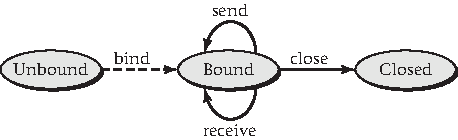
\includegraphics{hail_f0904}}
%\centerline{\def\epsfsize#1#2{0.6#1}\epsfbox{scan-9-3.eps}}
\caption{This state diagram shows the life cycle of datagram sockets used for sending or receiving UDP
  datagrams.  In the Java API, the class {\tt java.net.DatagramSocket} is
  used for this purpose, and binding happens automatically as part of
  the constructor.}
\label{scan-9-3}
\end{figure}
\begin{figure}
\centerline{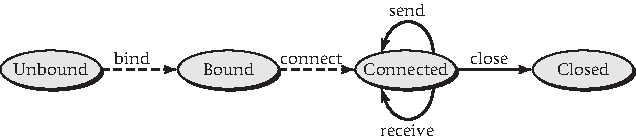
\includegraphics{hail_f0905}}
%\centerline{\def\epsfsize#1#2{0.6#1}\epsfbox{scan-9-4.eps}}
\caption{This state diagram shows the life cycle of client-side stream
  sockets used to initiate TCP connections.
  In the Java API, the class {\tt java.net.Socket} is used for this purpose,
  and binding and connection ordinarily both happen automatically as
  part of the constructor.}
\label{scan-9-4}
\end{figure}
\begin{figure}
\centerline{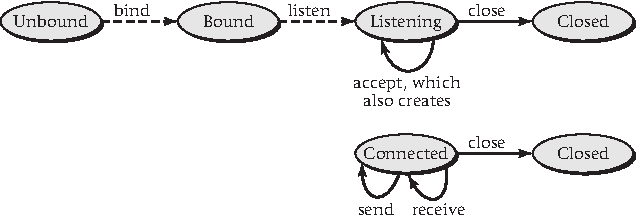
\includegraphics{hail_f0906}}
%\centerline{\def\epsfsize#1#2{0.6#1}\epsfbox{scan-9-5.eps}}
\caption{This state diagram shows the life cycle of server-side stream
  sockets used to accept TCP
  connections.  In the Java API, the class {\tt java.net.ServerSocket} is
  used for this purpose, and the bind and listen operations ordinarily
  are performed automatically as part of the constructor.  Each time
  the accept operation succeeds, a new connected socket is returned,
  which in the Java API is an instance of {\tt java.net.Socket}.}
\label{scan-9-5}
\end{figure}
The states are as follows:
\begin{itemize}
\item
When freshly created, the socket may be \vocab{unbound}, with no address or
port number.  In this state, the socket does not yet represent a
genuine communication endpoint but is just a hollow shell that has
the potential to become an endpoint once bound.  In the POSIX and
Winsock APIs, all sockets are created unbound and are then bound using
a separate operation.  In the Java API, you can create an unbound
socket if you really want to (and then later bind it), but the normal
constructors for the socket classes do the binding at the time the
socket is created, saving a step.
\item
A socket can be \vocab{bound} but neither connected nor listening for
incoming connection attempts.  For UDP, datagrams can be sent or
received in this state.  For stream sockets, this state is only used
as a stepping stone to the connected or listening state.  In the Java
API, the transition to the connected or listening state is generally
accomplished at the time the socket is created, whereas in the POSIX
and Winsock APIs, the connect and listen operations are explicit.
\item
A bound socket can be \vocab{connected} to a remote address and port number,
forming a TCP connection over which bytes can be streamed in each
direction.
\item
Alternatively, a bound socket can be \vocab{listening} for incoming connection
attempts.  Each time the application program accepts an incoming
connection attempt, the socket remains in the listening state.  A
new socket is spawned off, bound to the same local address and port
number as the original listening socket, but in the connected state
rather than the listening state.  The new connected socket can then be
used to communicate with the client that initiated the accepted
connection.

A server program can in this way wind up with lots of
sockets associated with the same local port number---one listening
socket and any number of connected sockets.  The TCP
connections are still kept distinct, because each TCP connection is
identified by four numbers: the internet addresses and port numbers on
both ends of the connection.
\item
Finally, a socket should be \vocab{closed} when it is no longer needed.  The
socket data structure becomes a vestige of the former
communication endpoint, and no operations can be legally performed on
it.
\end{itemize}

To illustrate how a TCP server accepts incoming connections and then
communicates using the resulting connected sockets, consider the Java
program in Figure~\ref{Server-code}.
\begin{figure}
\begin{verbatim}
import java.io.*;
import java.net.*;

class Server {
  public static void main(String argv[]) throws Exception {
    String storedMessage = "nothing yet";
    ServerSocket listeningSocket = new ServerSocket(2718);
    while(true) {
      Socket connectedSocket = listeningSocket.accept();
      BufferedReader fromClient = new BufferedReader
        (new InputStreamReader(connectedSocket.getInputStream()));
      PrintWriter toClient = new PrintWriter
        (connectedSocket.getOutputStream());
      String newMessage = fromClient.readLine();
      toClient.println(storedMessage);
      storedMessage = newMessage;
      toClient.close();
      fromClient.close();
      connectedSocket.close();
    }
  }
}
\end{verbatim}
\caption{This message-storage server listens on port 2718 for
  connections.  Each time
it gets one, it reads a line of text from the connection to use as a
  new message to store.  The server
then writes the previous message out to the connection.  For the first
connection, the message sent out is {\tt nothing yet}, because there is no
previous message to deliver.}
\label{Server-code}
\end{figure}
This server contains an infinite loop that 
accepts only one connection at a time, reading from that
connection, writing back to it, and then closing it before accepting
the next connection.  This would not be acceptable in a
performance-critical setting such as a web server, because a slow client
could hold all others up, as you can demonstrate in Exploration Project~\ref{single-threaded-server-demo}.  In Programming
Project~\ref{multithreaded-server-project}, you will modify the server
to spawn off a concurrent thread for each incoming client.  Even sticking
with the unmodified code, though, you can see that there may be many
sockets associated with port 2718 as the program runs: one listening
socket (of class {\tt ServerSocket}) that exists the whole time the server
is running, and a whole succession of connected sockets (of class
{\tt Socket}), one for each time a client connects.  In a multithreaded
version, several connected sockets could be in existence at the same
time, all on port 2718.

If you compile and run the Java code from Figure~\ref{Server-code},
you can test out the server in the same way as shown in
Section~\ref{http-section} for HTTP.  That is, you can use the
\verb|telnet| program to connect to port 2718 on whatever machine is
running the server, just as there I connected to port 80 on
\textit{www.gustavus.edu}.  Once you connect with \verb|telnet|, type in a line
of text.  You should see the {\tt nothing yet} response and then see the
connection close.  Connect again (from the same or a different
machine) and repeat the procedure.  This time you should see the line
of text you previously entered come back to you.  If you find you can't
connect to port 2718, there is probably a security firewall blocking your
connection.  The simplest workaround would be to limit yourself to testing
connections from the same machine that is running the server program; connect
using the special hostname \textit{localhost}.

Rather than using \verb|telnet| for the client side of this
interaction, you could use a program written specifically for the
purpose.  This would demonstrate the other way TCP sockets are used,
to connect from within a client program to a server's port.
\begin{figure}
\begin{verbatim}
import java.io.*;
import java.net.*;

class Client {
  public static void main(String argv[]) throws Exception {
    if(argv.length != 2){
      System.err.println("usage: java Client hostname msgToSend");
      System.exit(1);
    }
    String hostname = argv[0];
    String messageToSend = argv[1];
    Socket connectedSocket = new Socket(hostname, 2718);
    BufferedReader fromServer = new BufferedReader
      (new InputStreamReader(connectedSocket.getInputStream()));
    PrintWriter toServer = new PrintWriter
      (connectedSocket.getOutputStream(), true);
    toServer.println(messageToSend);
    String retrievedMessage = fromServer.readLine();
    System.out.println(retrievedMessage);
    toServer.close();
    fromServer.close();
    connectedSocket.close();
  }
}
\end{verbatim}
\caption{This client program receives a hostname and a
  textual message string as command line arguments. It connects to the server running on the
  specified host's port 2718 and sends it a line of text containing
  the message.  It then reads a reply line back and prints it out for
  the user to see.}
\label{Client-code}
\end{figure}
The program in Figure~\ref{Client-code} directly forms a connected socket, bound to an arbitrary
system-chosen port on the local host but connected to the specified
host's port 2718.  To try this program out, you could compile it and
then run a command like
\begin{verbatim}
java Client localhost test-message
\end{verbatim}
You should see in response whatever previous message was stored in the
server.  Moreover, repeating the command with a new message should
retrieve \verb|test-message|.

The preceding Java examples send only a single line of text in each
direction over each connected socket.  However, this is just a feature
of the example I chose; in effect, it defines the nonstandard
application-layer protocol being used.  The same TCP transport layer
(accessed through Java's socket API) could equally well carry any
number of lines of text, or other sequences of bytes, in each
direction.  You would just need to insert a loop at the point in the
program that reads from or writes to the connected socket.
For example, you could write an HTTP client or server in Java using
this sort of code.

\subsection{TCP, the Dominant Transport Protocol}\label{tcp-section}

You now understand how TCP can be used, through a socket API, to
provide reliable transport of a byte stream in each direction over a
connection between ports.  Now I can take you behind the scenes and
give you a brief overview of some of the techniques TCP uses to
support reliable ordered byte streams.  This will help you appreciate
some of the difficult performance-critical issues.  In this
subsection, I will sketch TCP in its most well-established form; these
TCP mechanisms are generally implemented within each operating system's kernel.
Recent enhancements, as well as proposals for further change, are the
topic of Section~\ref{post-tcp-section}.

As the application program uses the kernel's socket API to send bytes,
the kernel stores those bytes away in an internal buffer.  From time
to time, it takes a group of consecutive bytes from the buffer, adds a
header of identifying information to the beginning, and sends it over
the network to the receiver using the network layer, that is, IP.
The chunk of bytes with a header on the front is called a
\vocab{segment}.  Each connection has a maximum segment size,
typically no larger than 1460 bytes, exclusive of header.  Thus, if the application program
is trying to send a large number of bytes at once, the kernel will
break it into several segments and send each.  If the application
program is sending only a few bytes, however, the kernel will wait
only a little while for more bytes, and failing to get any, will send
a small segment.  One
performance bottleneck is the copying of bytes from the application
program to the kernel's buffer, and generally at least once more
before reaching the network interface card.  Systems optimized for
network performance go to great lengths to reduce the number of times
data is copied.

The header on each segment provides the port
number for each end of the connection.  It also specifies the
position the segment's bytes occupy within the overall sequence being
transmitted.  For example, the first segment header might say ``these
are bytes 1 through 1000,'' and then the second segment header would say
``these are bytes 1001 through 2000.''  The receiving code (also part of
an operating system kernel) needs to pay attention to these sequence
numbers and use them to deliver the bytes correctly to the application
program that is using the socket API to read the data.  Segments may
arrive over the network out of order, for example, by taking two
different routes.  Thus, the kernel needs to
store the arriving data in a buffer and return it to the application
program in the order of sequence numbers, not in the order it
arrives.  As on the sending side, the trick is to do this without
spending too much time copying data from one place to another.

In addition to arriving out of order, some segments may not arrive at
all, because the network layer may occasionally lose a packet.  To
overcome that problem, TCP has mechanisms for retransmitting segments.
The sender must continue to buffer each segment until its receipt is
acknowledged, in case it needs to be retransmitted.  Also, a segment
believed to be lost may be retransmitted, and then turn out to not
have been lost after all, but only delayed.  Thus, the receiver needs
to cope with duplicate segments.

Performance would be unacceptable if TCP transmitters sent only one
segment at a time, waiting for acknowledgment before sending another.
However, it would not be a good idea to allow arbitrarily many
segments to be sent without waiting for acknowledgment.  If a fast
computer were sending to a slow computer, the receive buffer space
could easily be overwhelmed.  Thus, one of the many features TCP
provides behind the scenes is \vocab{flow control}, which is to say,
a receiver-controlled limit on how much unacknowledged data the sender
is allowed to have outstanding at any time.

In traditional TCP, each acknowledgment contains a single number, $n$,
to indicate that bytes 1 through $n$ have been successfully received
and that byte $n+1$ hasn't been.  This style of acknowledgment, known
as \foldvocab{cumulative}{acknowledgment}, is rather limited.  Suppose the sender
transmits seven segments of 1000 bytes each and only the first,
third, fifth, and seventh arrive.  The receiver will see four incoming
segments and will send four acknowledgments, all saying bytes 1
through 1000 have been received. The sender will know that those bytes
were received and have a pretty good clue that bytes 1001 through 2000
were not.  It will also have a clue that three of the subsequent five
segments were received, but it will have no idea which three.

The preceding example illustrates one scenario under which a TCP
sender will retransmit a segment.  Having received an acknowledgment
of the first 1000 bytes and then three duplicates of that same
acknowledgment, the sender is justified in assuming the second segment
was lost and retransmitting it.  The rules of TCP specify waiting for
three duplicate acknowledgments, because one or two can easily occur
simply from segments arriving out of order.  That is, any duplicate
acknowledgment indicates a hole has opened up in the sequence number
order, but if segments are arriving out of order, the hole may quickly
get filled in without needing retransmission.

Unfortunately, to provoke the triple duplicate acknowledgment,
subsequent segments need to be transmitted.  If the sender has no more
segments to transmit, or is not allowed to send any more due to flow
control restrictions or the congestion control restrictions I will
describe shortly, then no duplicate acknowledgments will be triggered.
Thus, TCP senders need to fall back on some other means of detecting
lost segments; they use a timer.  If no acknowledgment is received in
a conservatively long time, then the segment is assumed lost.  This
conservative waiting period can cause substantial performance
degradation.

A final challenge for TCP is controlling congestion that occurs at the
switches (including routers) within the Internet.  Each link leading
out from a switch has a particular rate at which it can receive new
data.  Data destined for a particular outbound link may be coming into
the switch from any number of the inbound links.  If the total rate at
which that data is flowing into the switch exceeds the rate at which
it can be sent on the outbound link, then the switch will start to
build up a queue of data awaiting forwarding.  If the imbalance is
only temporary, the queue will build up a little, then drain back
down.  However, if the imbalance persists, then the queue will grow
long, creating lengthy delays, and then eventually get so full that
the switch starts discarding packets.  This phenomenon is known as
\vocab{congestion}.

Congestion is not good, because it causes packets of data to be delayed
or lost.  Because TCP interprets unreasonably long delays as packet
losses, either delays or outright losses can cause TCP to retransmit
segments.  This might even make the problem worse by sending more
data to the already congested switch.  Thus, TCP contains
congestion-control features, which act to throttle back the rate at
which it sends segments (new or retransmitted) when it detects packet
losses.  The theory is that most packet loss is caused by switches
with full queues and therefore can be interpreted as a sign of
congestion.

The details of congestion control are somewhat complicated.  The most
important facts to know are that it occurs independently in each TCP
connection, and that newly opened connections start with a very low
transmission rate, ramping up until the rate that causes congestion is
detected.  Thus, application performance can be improved by using
multiple TCP connections in parallel and by sending a lot of data over
each connection rather than repeatedly opening new connections for
a little data apiece.  Modern web browsers obey both these rules,
using parallel and persistent connections.  Parallel connections are
a mixed blessing, because they constitute an attempt to unfairly
compete with other Internet users, creating the potential for an
arms race.

\subsection{Evolution Within and Beyond TCP}\label{post-tcp-section}

Traditional TCP detects data loss through a combination of timeouts
and triple duplicate cumulative acknowledgments.  This detected data
loss serves as the sign of congestion.  TCP also responds to the
detected data loss with retransmissions in order to ensure that all
data is reliably delivered.  Every one of these three design
decisions has been challenged by networking researchers.  That is,
there are systems that detect loss in other ways, that detect
congestion other than through loss, and that ensure reliability other
than through retransmission.  Some of the results are already
partially deployed, whereas others remain research proposals.  Some
innovations also discard TCP's basic service model of the
bidirectional byte stream.  In this subsection, I will briefly
overview a few of these trends in order to make the point that
network protocols are not timeless truths, but rather are designs
that are subject to change.

As network hardware has improved, the rate at which bits can be
transmitted has greatly increased.  However, the time needed for those
bits to travel to the other side of the world and for acknowledgment
bits to travel back has not shrunk.  The consequence is that a
computer may now transmit quite a few bits before getting any
acknowledgment back.  As a result, it is now common to have large
numbers of unacknowledged TCP segments.  In this situation, the
weakness I mentioned for cumulative acknowledgment starts to become
significant.  There may well be more than one lost segment, and it
would be nice to know exactly which ones were lost.  For this reason,
a \foldvocab{selective}{acknowledgment} feature was added to TCP, in
which the receiver can provide the sender more complete information
about which bytes have been received.  This provides a new way to
detect data loss.

In whatever manner data loss is detected, it likely stems from congestion.  That
does not mean, however, that the TCP sender needs to wait for a lost
segment in order to sense congestion.  If it could sense the
congestion sooner, it could avoid the loss entirely.  One way
this can be done, deployed in some parts of the Internet, is for the
routers to provide \vocab{Explicit Congestion Notification}
(\vocab{ECN}).  That is, they send an overt signal to the TCP
transmitters to throttle back, rather than needing to implicitly code
that signal by discarding a packet.  Another approach, which has been
experimented with, is for the TCP sender to notice that
acknowledgments are starting to take longer and infer that a queue
must be building up.  This is called \vocab{TCP Vegas}.

Lost segments don't just signal congestion; they also prevent data
from being delivered, necessitating retransmissions.  However, there
is another approach to ensuring that all data is delivered, even if
some packets are lost. Namely, the data can be encoded into a
redundant format, in which any sufficiently large subset of the
packets contains enough information to allow all the data to be
reconstructed.  This concept is best explained by a highly
simplified example, shown in Figure~\ref{scan-9-6}.
\begin{figure}
\centerline{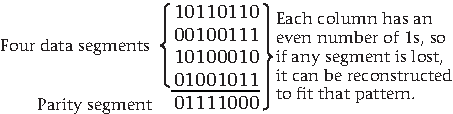
\includegraphics{hail_f0909}}
%\centerline{\def\epsfsize#1#2{0.6#1}\epsfbox{scan-9-6.eps}}
\caption{Sending redundant data allows loss to be tolerated.  Suppose four
  segments of data are to be sent; for simplicity, here each segment
  is only 1 byte long.  Suppose the loss rate is low enough that it is
  unlikely two segments will be lost.  Rather than waiting to see
  which one segment is lost, and then retransmitting it, a sender can
  transmit the four data segments and a parity segment,
  each with a sequence number in the header.  Any one of the five can
  be lost, and yet all four data segments will be deliverable, because
  the lost segment can be reconstructed.}
\label{scan-9-6}
\end{figure}
This general approach is known as \foldvocab{forward}{error
correction} using an \foldvocab{erasure}{code}.  More sophisticated
versions have been used to build high-performance systems for streaming
large files, such as videos, using UDP.

One final area of change is in the service provided by TCP.  An
alternative transport protocol known as \vocab{SCTP}
(\vocab{Stream Control Transmission Protocol}) is a proposed Internet
standard that would offer similar reliable delivery and congestion
control to TCP, but would go beyond the single bidirectional byte
stream.  An SCTP sender can transmit a stream of messages, that is,
entire chunks of data akin to UDP datagrams, and have them delivered
not only reliably and in their correct order, but also with the
boundaries between them preserved, rather than all run together into
an undifferentiated byte stream.  Moreover, the SCTP connection can
carry more than one stream in each direction.  The messages on each
individual stream are delivered in order, but a lost message on one
stream doesn't hold up the delivery of messages on other streams.
Unlike the trends mentioned previously, which affect only low-level
details, if SCTP becomes popular, it will be necessary to rethink the
APIs that constitute the interface between application programs and
operating systems.

\section{The Network Layer}\label{network-layer-section}

The network layer delivers a packet of data to the appropriate
destination computer on an internet.  In this section, I will
highlight a few aspects of this layer.  First, I will explain the
difference between the two versions of IP and
explain how addresses are structured for the currently dominant
version, IPv4.  Second, I will give an overview of how routers forward
packets along appropriate paths to reach their destinations.  Finally,
I will explain Network Address Translation (NAT), a technology that has
considerable utility, but which is at odds with the original
end-to-end architectural principle of the Internet.

\subsection{IP, Versions 4 and 6}\label{IP-section}

Each packet of data sent on the Internet has a header
formatted in accordance with the \vocab{Internet Protocol} (\vocab{IP}).  If the
packet contains a TCP segment or UDP datagram, the TCP or UDP header
follows the IP header.  Each packet starting with an IP header is known as an IP datagram.  Thus, an IP datagram can contain a UDP datagram.  Because this is confusing, I will stick with the word ``packet'' when discussing IP and reserve ``datagram'' for UDP.

The most important pieces of information in
the IP header are as follows:
\begin{itemize}
\item
The version of IP being used, which governs the format of the
remaining header fields; currently version 4 is dominant and version 6
is in limited use (version 5 does not exist)
\item
The internet address from which the packet was sent
\item
The internet address to which the packet should be delivered
\item
A code number for the transport-layer protocol, indicating whether the
IP header is followed by a TCP header, UDP header, or whatever else
\end{itemize}
Among the other header fields I will not discuss are some that support
optional extensions to the basic protocol.

The next-generation protocol, IPv6, differs from the currently dominant
IPv4 in two principle ways.  First, the source and destination
internet addresses are much larger, 128 bits instead of 32.  This
should greatly ease assigning internet addresses to ubiquitous devices
such as cell phones.  Second, IPv6 was designed to support security
features, protecting packets from interception, alteration, or
forgery.  However, these features have in the meantime become
available as an optional extension to IPv4, known as \vocab{IPsec}.
Partially for this reason, the transition to IPv6 is happening
exceedingly slowly, and IPv4 is still by far the dominant version.

As I explained in Section~\ref{networks-and-internets-section}, an
internet address contains two components: an identifier for a
particular network and an identifier for a specific interface on that
network.  (My analogy in that section was with ``Max Hailperin,
Gustavus Adolphus College.'')  Given that IPv4 addresses are 32 bits
long, you might ask how many of these bits are devoted to each
purpose.  For example, does the address contain a 16-bit network
number and a 16-bit interface number?  Unfortunately, the answer to
this question is not so simple.

Each IPv4 address has a prefix, some number of bits long, that
identifies the network, with the remainder of the 32 bits identifying
the interface within the network.  However, the length of the network
prefix varies from network to network, so that internet addresses are
not partitioned into their two components in a uniform way.
The motivation for this awkward design is that the Internet needs both
to support a large number of networks (more than $2^{16}$, for example)
and also some large networks (some containing more than $2^{16}$
interfaces, for example).

The conceptually simple solution to this problem would be to use larger
fixed-format addresses, perhaps containing a 32-bit network number and
a 32-bit interface number.  However, the designers of IPv4 decided to
stick with a total of 32 bits, because this address size was already
in place from an early fixed-format version of internet addressing, in
which the network identifier was always 8 bits long and the interface
identifier 24 bits.  The designers considered it more important to
stick with their prior address size, 32 bits, than with their prior
design concept, that the bits be partitioned in a uniform way.  Thus, they made the design choice to cram all
addresses into 32 bits by allowing a flexible division.  This allows
both for a small number of large networks (with short network
prefixes) and a large number of small networks (with long network
prefixes).

IPv4 addresses are conventionally written in \vocab{dotted
decimal} format, in which the 32-bit address is divided into four
8-bit components, and each of the 8-bit components is translated into
a decimal number.  The four decimal numbers are written with dots
between them.  As an example, my computer's internet address is
138.236.64.64.  Translating 138, 236, 64, and 64 from decimal to binary
produces 10001010, 11101100, 01000000, and 01000000.  Thus, my internet address
in binary is 10001010111011000100000001000000.

Of these 32 bits, the first 21 identify the network for my college's
department of mathematics and computer science, whereas the remaining
11 identify my specific computer on that network.  My computer's
operating system kernel is aware not only of its own internet address,
but also of this division into 21 bits and 11.  The latter fact is stored as a
\vocab{mask}, which in my case is 255.255.248.0.  If you translate
that from dotted decimal to binary, you will see that the first 21
bits are 1s, whereas the last 11 bits are 0s.

The kernel uses this information whenever it sends out an internet
packet.  It compares the destination address to its own address,
paying attention only to the prefix specified by the mask.  Thus, in
my case, the kernel checks whether the first 21 bits of the
destination address are the same as my own.  If so, the destination is
on my own network, and my computer's kernel should send the data
directly, using my network's own link-layer addressing mechanism.

If, on the other hand, the destination is outside my network, then the
kernel should send the packet to the \foldvocab{gateway}{router}
leading from my local network to the outside world.  At the link
layer, the kernel will send the packet out with the gateway router's
network address, though it will still have the ultimate destination's
internet address within the IP header.

\subsection{Routing and Label Switching}

In the ordinary functioning of the Internet, no entity actually
selects a route for a packet of data to follow, in the sense of
planning the entire route in advance.  Instead, each time the packet
arrives at a router, that router decides which neighboring router to
forward the packet to.  The overall route emerges as the composite
result of all these local decisions.

When a router needs to forward a packet, it decide which neighboring
router should be next by consulting its forwarding table.  Each entry
in the forwarding table specifies an internet address prefix and what
the next router should be for that prefix.  Given this large table,
the router's forwarding decision can be made rather rapidly, because it
just requires a table lookup.  The one problem is that the entries in
the table are keyed by variable-length prefixes, making the lookup
operation more complicated than would be the case with fixed-length
keys.

One other limitation of traditional internet routing, beyond the need
to look up variable-length prefixes, is that all traffic for the same
destination network gets forwarded to the same next router.  Large
service providers in the core of the Internet would prefer more
flexible traffic engineering with the ability to send some of the
traffic through each of several alternative routes.  These same core
providers are also the ones for whom expensive lookup operations on
variable-length prefixes are most burdensome, because their routers need
to switch traffic at a very high rate.

In order to address both these issue, some Internet service providers,
particularly in the core of the Internet, are moving away from
traditional IP routers to \foldvocabs{label switching}{router} using
\vocab{Multiprotocol Label Switching} (\vocab{MPLS}).
A label switching router looks up the next router, not using a
variable-length prefix of the destination address, but instead using a
fixed-length label that has been attached to the packet; MPLS
specifies the standard format for this labeling.

When an IP packet first reaches a label switching router, the router
attaches a label to it based on both the destination address and any
traffic engineering considerations.  Once the packet is labeled, it
can be forwarded from label switching router to label switching router
any number of times, based only on the label.  When the packet is
finally passed to a traditional router, the label gets stripped off.

With either approach, the performance-critical task of a router is
forwarding individual packets based on a table lookup operation.
However, the routers are also engaged in another less time-sensitive activity.
Namely, the
routers are constantly rebuilding their forwarding tables to reflect
the most recent information they have about the Internet.  They
exchange information with one another using routing protocols.  The
study of routing protocols, and of approaches to generating forwarding
table entries, is quite interesting, but I will leave it for networking
texts.

\subsection{Network Address Translation: An End to End-to-End?}
\label{nat-section}

Like many people, I have a network within my home, which uses the
Internet Protocol.  Moreover, from any of the computers on this
network, I can open a TCP connection to any computer on the Internet.
For example, I can browse any web site.  However, my home network is not
a constituent network of the Internet.  This situation, which is actually quite typical
for home networks, results from my use of \vocab{Network Address
Translation} (\vocab{NAT}) within the router that connects my home
network to my service provider's network.  NAT is a technology that
allows an entire network (or even an entire private internet) to pose
as a single computer on the Internet.  No matter which of my home
computers connects to an external site, the external site will see the
same source internet address, the one address that represents my whole
network.

Each computer on my home network has its own private IP address; for
example, one is 192.168.0.100 and another is 192.168.0.101.  All
packets on my home network use these addresses.  However, as the
router forwards packets out from the home network to the service
provider, it modifies the packets, replacing these private IP addresses
with the single public internet address my service provider assigned
me, which is 216.114.254.180.

If all the NAT router did was to change the packets' source addresses,
chaos would result.  Recall that each TCP connection is uniquely
identified by the combination of four values: the source and destination
addresses and port numbers.  Suppose I start browsing \textit{www.gustavus.edu}
on one home computer at the same time my wife does so on another of
our home computers.  Each of us is therefore opening a TCP connection
with destination address 138.236.128.22 and destination port number
80.  My source address starts out as 192.168.0.100, and my computer
picks a source port number it is not otherwise using, perhaps 2000.
My wife's source address starts out as 192.168.0.101, and her computer
also picks a source port.  Perhaps by coincidence it also picks 2000.
Within our home network, our two TCP connections are distinguishable
because of our two different IP addresses.  However, outside the home
network is another issue.  If the NAT box rewrites our packets so both
have source address 216.114.254.180 and leaves both our port numbers
as 2000, then it will have combined what should have been two separate
TCP connections into one.

To get around this problem, the NAT router rewrites our packets'
source port numbers (in the TCP headers) as well as the source
addresses (in the IP headers).  Internally to our network, we have
distinct addresses but may have coincidentally identical port
numbers.  Externally, we share a common address, but the NAT router
makes sure we use different port numbers.  For example, it might
assign me port number 3000 and my wife port number 4000.  Thus, the
router would make two entries in a table for its own later reference.
One entry would show that it should map all internal packets destined
for the web server from
address 192.168.0.100 and port number 2000 into external packets with
address 216.114.254.180 and port number 3000.  The other entry would show
that traffic to the web server from internal address 192.168.0.101 with port number 2000 maps into
external address 216.114.254.180 with port number 4000.
Figure~\ref{scan-9-8}
\begin{figure}
\centerline{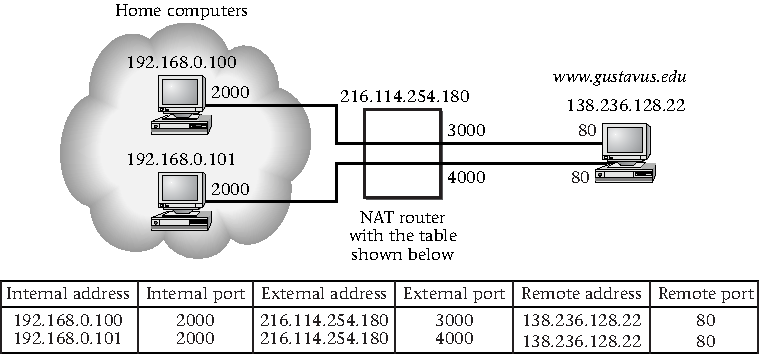
\includegraphics{hail_f0910}}
%\centerline{\def\epsfsize#1#2{0.6#1}\epsfbox{scan-9-8.eps}}
\caption{A NAT router rewrites port numbers as well
  as addresses so two computers can share a single public address.}
\label{scan-9-8}
\end{figure}
illustrates this scenario.

Luckily, port numbers are not a scarce resource.  The TCP header
fields for source and destination port numbers are each 16 bits in
size, yet computers do not ordinarily use anywhere near $2^{16}$ ports
apiece.  Therefore, the NAT router has no problem assigning distinct
external port numbers for all the ports in use by any of the computers
on the home network.

The NAT router has one further essential function.  It must also rewrite
in the reverse manner each packet coming in from the Internet at large
to the private network.  For example, if a packet arrives with
source address 138.236.128.22, source port 80, destination address 216.114.254.180, and destination port 3000,
then the NAT's table will show that this belongs to my connection, and
so the NAT will modify the packet to show destination 192.168.0.100
with port 2000.  By the time the packet reaches my computer, it will
look as though the web server was directly communicating with me using
my private address.

What happens if an external computer wants to initiate a TCP
connection to one of my home computers?  In the particular case of my
home, it is out of luck.  My NAT router is configured to forward only
inbound packets that come as part of a connection initiated from the
private network. However, the answer might be somewhat different on
another network using a NAT router.  Consider, for example, a business
that chooses to use a NAT router.
The business would allow outgoing connections from all its computers,
just as I do at home.  These outgoing connections would create
temporary entries in the router's table of rewriting rules, just like
in my router.  However, the business would also allow incoming
connections to port 80 (the standard HTTP port) for its main web
server and to port 25 (the standard SMTP port) for its main email
server.  It would do this by configuring the NAT router with two
permanent rewriting rules.  Any packets coming to the business's
public address on port 80 should get rewritten to the web server's
private address, while retaining port 80.  Any packets coming to the
public address on port 25 should get rewritten to the email server's
private address, while retaining port 25.

This example illustrates one of the problems with NAT routing,
stemming from its violation of the end-to-end principle.  Suppose
someone within the business wants to start offering a new kind of
Internet service using a new application-layer protocol that listens
on a new port number.  For this to work, the corporate network
administrator would need to make a new entry in the NAT router's
table, like the two for the web and email servers.  This is a
significant stumbling block for introducing new services.  This is one
reason why many services today are packaged inside HTTP traffic,
directed to the usual port 80.

NAT routing has other problems as well.  One of the fundamental ones
is that IPsec is designed to prevent packets from being altered in
transit, but NAT relies on doing exactly that.  A technique for
working around this difficulty has recently been developed, but it
does at least introduce additional complexity.

Despite these problems, NAT routing is heavily used and becomes more
so every day.  The principle reason is that internet addresses are
expensive and so are worth sharing.  The negative consequences are
ameliorated by the fact that most network administrators would prefer to
put most internal computers off limits to external access anyhow, for
security reasons.

\section{The Link and Physical
  Layers}\label{link-physical-layers-section}

When you plug an Ethernet cable into a socket, the plug snaps into the
socket because it is the right size.  When your computer starts
sending high and low voltages over that cable, they are high enough
and low enough to be recognized as 1 and 0 by the equipment on the
other end, but not so extreme as to fry that equipment.  These are
examples of issues addressed by the physical layer.  Various physical-layer
standards exist for Ethernet over fiber optics, Ethernet over twisted
pairs of copper wires, and so forth.

Even granted that the physical layer can get bits from one end of a link to the
other, there are still problems to solve.  For example, how do
computers on the local network address data to each other?  Presumably,
each chunk of data (known as a \vocab{frame}) needs to have a header
that specifies a source address and destination address.  However, suppose
you plug a computer into a network, and it starts immediately hearing
1s and 0s, having come in on the middle of a frame.  It should start
paying attention at the start of the next frame.  How can it recognize
the boundary between frames?  Perhaps there is some definite minimum
space of silence between frames or some recognizable signal at the
beginning of each frame.  Shared
links (like radio channels) pose another problem: how can the various
computers take turns, rather than all transmitting at once?  These
issues of addressing, framing, and taking turns are concerns at the
link layer, which is also sometimes known as the data link layer.

Computer systems have hardware devices that support both the link and
physical layers.  The operating system kernel provides this hardware
with a frame of data to deliver, complete with the address of the
recipient on the local network.  The hardware does the rest.
Conversely, the hardware may interrupt the operating system to report
the arrival of an incoming frame.

Most of the issues at the link and physical layer have no direct
bearing on operating systems or other software.  The biggest exception
is addressing.  The two common kinds of networks (Ethernet and Wi-Fi)
use 48-bit addresses that are totally independent from the 32-bit
internet addresses.  Thus, whenever the operating system sends out a
packet of data to an internet address, and the address's prefix shows
that it is on
the local network, the kernel needs some mechanism for looking up the
corresponding 48-bit hardware address, commonly known as a
\vocab{MAC (Media Access Control) address}.

The kernel discovers MAC addresses using a network protocol called
\vocab{ARP} (\vocab{Address Resolution Protocol}).  The kernel
broadcasts a request to all machines on the local network asking if
any of them knows the MAC address corresponding to a particular IP
address.  The operating system kernels on all the receiving machines
compare the requested address to their own.  The one that sees its own
IP address responds, providing its own MAC address.  The requesting
kernel stores the information away in a table for later reuse, so that
it won't need to bother all other computers repeatedly.

Lots of network technologies have been developed, but two account for
the bulk of networks today.  Most networks that use wires or fiber
optics use some version of the Ethernet standard, whereas most
networks that use radio signals use some version of the Wi-Fi standard.
(Wi-Fi is also frequently known by the less-catchy name 802.11, which
is the identifying number of the working group that standardizes
it.)  Because these two use the same high-level interface, they can be
integrated into combined networks, in which any device can communicate
with any other device by MAC address, even if one is on the Ethernet
portion of the network and the other on the Wi-Fi portion.  Internet
routing is not required.  The switching devices that link Ethernet and
Wi-Fi in this way are known as \vocabs{access point}.

\section{Network Security}\label{network-security-section}

Just as networking is a large field that I can only survey in this chapter, network
security is a large area.  My purpose in addressing it here is
twofold.  First, I want to impress upon you how important it is; if I
remained silent, you might think it was unimportant.  Second, by
scratching the surface, I can give you some feel for some of the
constituent topics.

Data security must extend beyond security for the systems on which
the data is persistently stored.  In today's world, the data is frequently also in transit
over networks.  For example, my students' grades are not only stored
on the college's computer, they are also transmitted over the Internet
every time I do grading from home.  Thus, to be comprehensive, data
security must include network security.

There are two key differences between persistent storage and network
communication, however:
\begin{itemize}
\item
Large amounts of data are available for long periods of time in
persistent storage.  Networks, on the other hand, generally carry any
particular piece of data very fleetingly.  Contrast gaining access to
a merchant's database, containing all its customers' credit card
numbers, with tapping into the network connection and snagging the few
numbers that pass through during the time your interception is in
operation.
\item
Persistent storage is directly accessible only to a very limited
number of people who have physical access and who are subject to the
risks of being physically apprehended.  The Internet, on the other
hand, is accessible to an entire world worth of malefactors, many of
whom may be beyond effective reach of law enforcement.
\end{itemize}

When the Internet was less pervasive, the first of these factors was
the dominant one, and network security was not such a major concern.
Today, the second factor must be considered the dominant one.  Keep in
mind also that network adversaries are not limited to eavesdropping on,
or modifying, data already passing through the network.  They can also
send messages that might trigger additional data flows that would not
otherwise occur.  Many computers (typically in homes) today are
``owned'' by network intruders.  That is, the intruder has obtained
complete control and can remotely command the computer to carry out
any action, as though it were his or her own computer, including
accessing any of the persistently stored data.  The only way
organizations such as companies and government agencies prevent their
computers from being similarly ``owned'' is by devoting large amounts
of attention to network security.

\subsection{Security and the Protocol Layers}

Security vulnerabilities and threats exist at each layer of the
protocol stack.  Similarly, defensive measures are possible at each
level, whether to protect the confidentiality of transmitted data, or
to ensure the authenticity and integrity of arriving data.

Many of the most notorious network security problems have been at the
application layer.  Examples include forged email and the SQL Slammer
worm, which propagated by overflowing the memory space a particular
application program used for incoming messages.  Some of the
application-layer vulnerabilities stem from fundamental protocol
design decisions (such as that email can claim to come from anyone),
whereas others come from implementation flaws (such as a program not
checking whether it was putting more data into a buffer than it had
room for).

These vulnerabilities can be combated directly by using better
designs and more careful programming.  However, it is unrealistic to
expect perfection in this area, any more than in other human
endeavors.  Therefore, indirect methods should also be used to
minimize risk.  Section~\ref{fw-ids-section} mentions the role
well-configured firewall and intrusion detection systems can play.  To
take one example, there was essentially zero need for organizations to
allow traffic to come in from the Internet at large to the particular
port number used by the SQL Slammer worm.  This application-layer
vulnerability ought to have been shielded by a firewall.

The application layer also provides plenty of opportunity to actively
enhance security.  For example, the email protocols can be retrofitted
with cryptographic techniques to ensure that messages really come from
their stated sender, have not been modified in transit, and are
read only by their intended recipient; \vocab{PGP} (\vocab{Pretty Good
  Privacy}) and \vocab{S/MIME} (\vocab{Secure/Multipurpose Internet
  Mail Extensions}) do
exactly that.  To take another example, there is no reason why web
browsers and web servers need to directly send HTTP messages over
vulnerable TCP connections.  Instead, they can interpose a layer of
encryption known as the \vocab{Secure Sockets Layer} (\vocab{SSL}).
Every time you visit a secure web site and see the padlock icon click
shut, it means that SSL is in use.  Conceptually this is between the
main HTTP application layer and the TCP transport layer, but strictly
speaking it is an application-layer protocol.

At the transport layer, TCP is subject to its own set of
vulnerabilities.  Many of the denial-of-service attacks on network
servers take place at this level; the server under attack is flooded
by initial connection-establishment requests that are never followed
up on.  Proposals for
fixing that problem in fundamental ways run into the difficulty of
changing any protocol that is so widely deployed.

One example of a security-enhancement technology at the transport
layer is an optional TCP feature for message authentication.  This
feature is particularly used by routers in order to secure their
communication with neighboring routers.  If it were possible for an
intruder to inject bogus routing information, the Internet could be
rendered unusable.  Therefore, routers ``sign'' their routing update
messages, using the optional TCP feature, and check the signatures on
the updates they receive from neighboring routers.

One of the biggest security vulnerabilities at the network layer is
that packets may have incorrect source addresses.  The typical response to
this problem is filtering at routers.  For example, no packets should
be allowed out of my college campus onto the Internet at large if the
source address is not a legitimate one from the range assigned to this
college.  That would prevent someone here from pretending to be
elsewhere.

I already mentioned that IPsec is a security technology at the network
layer.  The most common application of IPsec is when an organization
has computers at several physical locations (including, frequently,
within workers' homes) and wants to allow them all to communicate
securely with one another, even though the traffic between locations
is carried on the public Internet.  IPsec supports this kind of
\vocab{virtual private network} (\vocab{VPN}) by making sure every
packet of data sent is encrypted, so as to be completely opaque to
eavesdroppers, and so as to stymie any active intruder who would attempt
to modify or inject packets.

Finally, the lowest layers of the protocol stack, the link and
physical layers, are not immune from security issues.  I will mention
just two.  One is that the ARP protocol, used to translate internet
addresses into MAC addresses, was designed without any serious
consideration of security issues.  As a result, it is easy for any
computer on a local network to take over an internet address that
ought to belong to another computer on the same network.  This is an
attack more readily detected and responded to than prevented.  To take
a second example, Wi-Fi signals for many organizations can be picked
up from the street outside.  Moreover, the encryption built into early
versions of Wi-Fi was faulty and even in newer versions is frequently
not turned on.  If you use Wi-Fi, you should definitely read one of
the widely available tutorials on Wi-Fi security.  These systems can
be configured much more securely than they usually are.

\subsection{Firewalls and Intrusion Detection
  Systems}\label{fw-ids-section}

A \vocab{firewall} is a system that imposes some restriction on the
Internet traffic crossing a border, for example, between a company and
the outside world, or between a particular computer and the rest of
the Internet.  Security-conscious organizations deploy multiple
firewalls, protecting not only the outer perimeter, but also the
borders between internal groups and around individual systems.  Every
computer installation that is hooked up to the Internet, even as small
as a single home computer, should have at least one firewall.

A firewall can be a computer (or special-purpose hardware unit) devoted
to the purpose, a router that has been configured to filter traffic,
or software installed directly on the computer being protected.  If
the firewall operates correctly, any of these approaches is valid.
However, if the firewall software itself is buggy, the consequences
are likely to be more severe if it is operating on the same computer
that is being protected.  The best practice is to use a reputable
external firewall at the organizational and workgroup perimeters and
then software firewalls on individual computers.  Home users should
ideally use the same approach.  The external firewall in this case may
be a NAT router.

The big problem with firewalls is configuring them to let through only
traffic that has a good reason to exist while blocking all other
traffic.  Empirical studies have shown that a large percentage of
firewalls are misconfigured.  Security-conscious organizations have
their firewall configuration files examined by auditors and also have
penetration testing performed, in which the auditors make attempts to
gain access to the protected network.

In an organizational setting, there is pressure on network
administrators to not configure firewalls too restrictively.  If
traffic necessary to the organization's functioning is blocked,
someone will complain.  These complaints could cost the administrator
a job.  In a home setting, on the other hand, you are likely to be
complaining to yourself and can presumably stand the heat.
Therefore, you should set all firewall settings as restrictively as
possible, and wait and see what harm it does you.  Loosen up on
only those settings that prove to get in your way.  This approach
compensates for your inability to hire security auditors.

One of the most important steps an organization can take to preserve
overall security is to use firewalls to isolate machines that are
exposed to attack, so that even if those particular machines are
``owned'' by attackers, the damage is limited.  As an example,
consider a web server that does not support interactive transactions
(such as shopping), but rather just disseminates information about the
organization.  A security-conscious configuration is as shown in
Figure~\ref{scan-9-9}.
\begin{figure}
\centerline{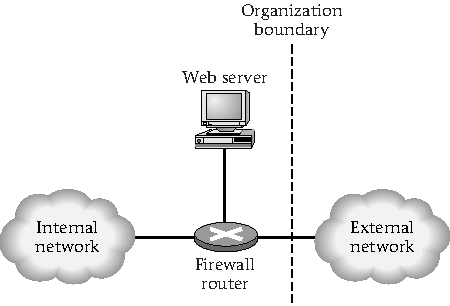
\includegraphics{hail_f0911}}
%\centerline{\def\epsfsize#1#2{0.6#1}\epsfbox{scan-9-9.eps}}
\leftline{Configuration of the firewall router:}
\centerline{\begin{tabular}{|c|c|c|}
\hline
\bf Initiator & \bf Target & \bf Allowed
ports\\\hline\hline
external network & web server & 80\\\hline
internal network & web server & a few needed for operation\\\hline
internal network & external network & none\\\hline
external network & internal network & none\\\hline
web server & any & none\\\hline
\end{tabular}}
\caption{This firewall configuration allows an organization's web
  server to provide static content to the outside world but allows
  for no other interaction. An organization with other needs would have other
  equally security-conscious modules added to this one.}
\label{scan-9-9}
\end{figure}

Suppose that the web server software has some bug, such that by
sending some clever, over-long message to the server's normal port
80, an outside attacker can overwrite some critical memory and come to
``own'' the server, executing arbitrary code.
Depending on the access controls in place on the server,
the attacker
may be able to deface the web site, replacing the organization's web pages with
others.  However, the attacker cannot mount any attack from the server
to other machines, whether on the internal network or the external,
because the firewall prohibits any outbound connections from the
server.  When employees of the organization want to reconfigure the
server or put new information on it, they do so using connections they
initiate from within the internal network.

In addition to firewalls, all organizational networks should also
include an \vocab{intrusion detection system} (\vocab{IDS}).  This
system monitors all network traffic looking for activity that does not
fit the usual, legitimate patterns.  The IDS can play two roles, both
alerting the network administrators to the existence of a problem and
capturing forensic evidence useful in crafting an appropriate
response.  The response can be both technical (such as removing an
infected machine from the network) and non-technical (such as
cooperating with law-enforcement officials).  A properly configured
IDS should protect not only against intrusions that breach the
organizational perimeter, but also against attacks mounted by insiders.

\subsection{Cryptography}

Cryptography consists of mathematical techniques for transforming data
in order to assure confidentiality or integrity and authenticity.
Cryptography underlies much of network security, ranging from
application-layer secure email and web browsing to link-layer
encryption within the Wi-Fi protocol.  Cryptography provides the means
for legitimate communication to continue even as adversaries are
thwarted.  However, you should be aware that most practical security
problems are outside the scope of cryptography.  Rarely is there a
report of encryption being broken, whereas misconfigured
firewalls and systems vulnerable to buffer overflows are everyday
occurrences.

Cryptographic techniques can be categorized in two independent ways:
\begin{itemize}
\item
Some techniques rely on both the sender and the receiver knowing a
\foldvocab{shared}{secret}, that is, a secret key that the two of them
both know but intruders don't.  Other techniques use a \vocab{key
pair}, with one component known to the sender and the other to the
receiver.  These two options are known as
\foldvocab{symmetric-key}{cryptography} and
\foldvocab{asymmetric-key}{cryptography}.  Because in many
applications one half of a key pair can be made publicly known while
the other is kept secret, asymmetric-key cryptography is also known as
\foldvocab{public-key}{cryptography}.
\item
Some techniques \vocab{encrypt} the message, that is,
transform the message so that it is not readable
without the appropriate key, whereas other techniques leave the
message itself alone but append a \vocab{Message Authentication Code}
that allows the possessor of the appropriate key to verify that the
message really comes from the legitimate sender and was not modified.
Note that the abbreviation \vocab{MAC} is used in this context independently
from its use in describing features of link-layer protocols, such as MAC
addresses.
\end{itemize}

The more bits long a cryptographic key is, the more work the
legitimate sender and receiver need to do, but also the more work any
intruder needs to do.  The goal in designing a cryptographic system is
to make the legitimate parties' work scale up only modestly with key
size, whereas the intruder's work scales up much more rapidly.  That
way, a key size can be chosen that is infeasible for an intruder to
break, yet still practical for use.  Unfortunately, none of the
computational hardness results used in practical cryptosystems have been proved.
Thus, the possibility remains that a sufficiently clever intruder
could find a way to break the system that does not scale up so rapidly
with key size.

Symmetric-key systems of reasonable security are more computationally
efficient for the legitimate parties than asymmetric-key systems are.
However, giving each potential pair of communicating parties a shared
secret in advance is impractical.  Thus, many practical systems (such
as PGP and SSL) combine the two types of cryptography, using asymmetric-key cryptography to
establish a secret key and then switching to symmetric-key
cryptography for the bulk of the communication.

The present standard
technique for symmetric-key encryption is \vocab{AES}
(\vocab{Advanced Encryption Standard}), also known as \vocab{Rijndael}.  Many applications still use the
prior standard, the \vocab{Data Encryption Standard} (\vocab{DES}).
However, DES is now considered not very secure, simply because the key
size is too small.  A more secure variant, \vocab{3DES}, uses the
basic DES operation three times.  Best practice for new applications
is to use AES.

The most well-known technique for asymmetric-key encryption is the
\vocab{RSA} system, named for the initials of its three developers,
\index{Rivest, Ronald L.}Rivest, \index{Shamir, Adi}Shamir, and \index{Adleman, Leonard M.}Adleman.  Data transformed with one half of the
RSA key pair can be transformed back to the original using the other
half of the key pair; the two specify inverse functions.  Thus, a user
who wants to receive encrypted messages can make one half the key pair
public for any sender to use, while keeping the other half private so
that no one else can read the messages.

The standard technique for computing a MAC using a shared secret is
known as a \vocab{Hashed Message Authentication Code}
(\vocab{HMAC}).  The shared secret and the message are combined together
and fed into a \foldvocab{cryptographic}{hash function}, also known as
a \vocab{message digest function}.  This function is designed so that
adversaries cannot realistically hope to find another input that
produces the same output.  Thus, if the recipient's copy of the
message and shared secret result in the same HMAC code, the recipient
can be confident that the message is legitimate, because it came from
someone else who knew the same two ingredients.  As an additional
safeguard against certain possible flaws in the cryptographic hash
function, the standard HMAC technique (used in IPsec, for example)
applies the hash function twice, as shown in
Figure~\ref{scan-9-10}.
\begin{figure}
\centerline{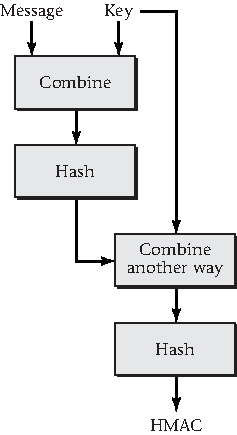
\includegraphics{hail_f0912}}
%\centerline{\def\epsfsize#1#2{0.6#1}\epsfbox{scan-9-10.eps}}
\caption{An HMAC can be computed as shown here.  Both the sender and
  the receiver use this computation, each with its own copy of the
  shared secret
  key.  The sender uses the message it is sending and transmits the
  resulting HMAC along with the message.  The
  receiver does the computation using the (hopefully unchanged) message it received.  If all
  is well, the receiver computes the same HMAC as it received along with
  the message.}
\label{scan-9-10}
\end{figure}

HMAC codes are commonly based on one of two cryptographic hash
functions, \vocab{MD5} (\vocab{Message Digest 5}) and \vocab{SHA-1}
(\vocab{Secure Hash Algorithm 1}).  Unfortunately, neither of these
widely deployed functions turns out to be as secure as previously
thought.  Unlike DES, which simply used an insufficiently long key,
MD5 and SHA-1 have fallen prey to fundamental mathematical progress.  The
computational problem faced by adversaries does not scale up as
rapidly with hash size as had been conjectured, especially for MD5.  No one has yet found
a way to exploit these functions' vulnerabilities within the context
of HMAC.
However, the fact that the underlying cryptographic hash functions are weaker than previously thought is
worrisome enough that new systems should definitely at a minimum use SHA-1 rather
than MD5, as MD5's vulnerabilities are more pronounced.  System developers should monitor further news from the
cryptography research community and should consider using successors
to SHA-1, such as SHA-512.  Existing systems using MD5 (particularly in non-HMAC
contexts) should be reconsidered, and many of them should be converted
to SHA-1 or successor functions with deliberate speed.  Practical
exploits have been found for MD5's vulnerabilities in some
non-HMAC contexts; the same is not currently true for SHA-1.

The most common technique for creating an asymmetric-key MAC combines
a cryptographic hash function with the RSA system.  These MACs are
also known as \foldvocabs{digital}{signature}, because they share some
important features with real signatures, as I will discuss in the next
paragraph.  First, though, let me explain how they are computed.
Recall that each RSA key pair specifies a pair of inverse functions.
A sender can keep one half the key pair secret, for use in signing
messages, and make the other public, for use in checking messages.
Call the two inverse functions $S$ and $C$, for signing and checking,
and the cryptographic hash function $H$.  Then a sender can use
$S(H(m))$ as a signature for the message $m$. Any recipient who wants to
check this signature runs it through the function $C$, producing
$C(S(H(m)))$, which is the same as $H(m)$, because $C$ is the inverse
function of $S$.  The recipient also runs the received message through
$H$, and verifies that the same value of $H(m)$ results.  This
provides evidence that the message wasn't tampered with, and was
signed by the one person who knew $S$.  This system is summarized in
Figure~\ref{scan-9-11}.
\begin{figure}
\centerline{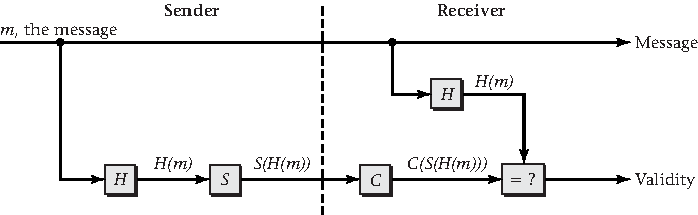
\includegraphics{hail_f0913}}
%\centerline{\def\epsfsize#1#2{0.6#1}\epsfbox{scan-9-11.eps}}
\caption{A digital signature is computed and verified as shown here.  The signing and
checking functions $S$ and $C$ are inverses, one kept private and the
other publicly known.  The role of the cryptographic hash function,
$H$, is simply to efficiently reduce the amount of data that $S$ and
$C$ need to process.}
\label{scan-9-11}
\end{figure}

The key difference between a digital signature and an HMAC is that the
recipient is in no better position to forge a digital signature than
anyone else would be.  Thus, digital signatures offer the feature
known as \vocab{non-repudiation}.  That is, if you have an embarrassing
email signed by me, you could show it to a third party and I couldn't
convincingly claim that you forged it yourself.  An HMAC, on the other
hand, would offer no evidence to a third party regarding which of the
two of us wrote the message.

\section*{Exercises}

\begin{chapterEnumerate}
\item
Under the end-to-end principle, which protocol layers are processed by
devices within the Internet, excluding the endpoint computers?
\item
List at least five types of header lines that can be used in the HTTP
protocol.  What is the function of each?
\item
What is one reason a domain name might take much longer to resolve the first time it
is used than on subsequent uses?
\item
Figure~\ref{scan-9-6} on page~\pageref{scan-9-6} illustrates how parity can be used as a
primitive form of erasure coding for forward error correction.  Show
how the third segment could be reconstructed if it were missing.
Also, suppose the parity segment were 01100001.  What would the
missing third data segment then have been?
\item
TCP and UDP headers contain port numbers used by the transport-layer
software to demultiplex incoming data to the appropriate
application-layer consumer.  What analogous number is in the IP header,
allowing the network layer to demultiplex to the appropriate
transport-layer consumer?
\item
Express the IP address 10100011000101000110000100001111 in dotted
decimal.
\item
Express the IP address 194.79.127.10 in binary.
\item
If a network mask is 255.255.192.0, how many bits long is the network prefix?
\item
If a network mask is 255.255.224.0, how many bits long is the network prefix?
\item
What would the network mask be for a 20-bit network prefix?
\item
What would the network mask be for a 22-bit network prefix?
\item
My computer has IP address 138.236.64.64 and mask 255.255.248.0.  For
which of the following destination IP addresses does my computer send the packet
directly, and for which does it send by way of the gateway router?
\begin{enumerate}
\item
138.236.71.64
\item
138.236.72.64
\item
138.236.64.72
\item
216.114.254.180
\end{enumerate}
\item
Identify by name and number which layer of the OSI reference model corresponds to each
of the following specific protocols, technologies, or functions:
\begin{enumerate}
\item UDP
\item retrieving email
\item Ethernet MAC addresses
\item IP
\item congestion control
\item fiber optics
\item TCP
\item routers
\item delivering bytes in their proper sequence
\item DNS
\item end-to-end flow-control
\item HTTP
\item retransmitting data for which no acknowledgment is received
\item CIFS
\item verifying that a cached web page is up to date
\item port numbers
\item NFS
\end{enumerate}

\item
Section~\ref{tcp-section} explains how TCP recovers from lost data segments, but it doesn't consider lost acknowledgments.  Nonetheless, the description in that section is sufficient that you could figure out how lost acknowledgments are tolerated.
\begin{enumerate}
\item
Explain why sometimes a lost acknowledgment is tolerated without any additional communication or delay.
\item
Explain why under other circumstances, TCP incurs extra delay and communication in recovering from a lost acknowledgment.
\end{enumerate}

\end{chapterEnumerate}

\section*{Programming Projects}

\begin{chapterEnumerate}
\item
\label{multithreaded-server-project}
Modify the message storage server from Figure~\ref{Server-code} on
page~\pageref{Server-code} so
that each accepted connection is handled in a separate thread, with
the main thread immediately looping back around to accept another
connection.  Using \verb|telnet|, show that a client that is slow
providing its line of text does not prevent other clients from being
served.  Your program should use a synchronized method that atomically stores a
newly arrived message and retrieves the previously stored message.
\item
Write a program that can retrieve a single file from a web server
using HTTP, given the hostname of the server and the name of the
file on the server. (For example, given \textit{www.gustavus.edu} and
\verb|/+max/|, it would retrieve my home page.)  You should directly
use a socket API, rather than any higher-level mechanism that already
implements HTTP for you.  Your handling of errors and other
exceptional circumstances can be very primitive, at least initially.
\item
The Java class {\tt java.net.ServerSocket} provides two methods called {\tt
  getLocalAddress()} and {\tt getInetAddress()} that can be used to
  find the local and remote internet addresses associated with a
  connected socket.  Write a server program that accepts connection
  requests and, each time it receives a connection, writes out on the
  connection a line of text containing the string form of the remote
  address from which the connection was received.  Write a client
  program that connects to the server, displays the string the server
  sends, and also displays the client's own local address.  Show how
  you can use this pair of programs to test whether the client is
  connected to the server through a NAT router or not.
\end{chapterEnumerate}

\section*{Exploration Projects}
\begin{chapterEnumerate}
\item
\label{dns-exploration-dig}
Most UNIX and Linux systems have a program named \verb|dig| that can
be used to send DNS queries and show the responses in human-readable
form.  Use this tool to explore the DNS.  For example, find the
internet addresses of some of your favorite computers, check whether
the CNAME chain leading from \textit{www.gustavus.edu.} still has the
same structure as I reported, and use the zone transfer function to
display the contents of your local zone.  What aspects of the DNS
do you find that were not mentioned in my description?

\item
\label{dns-exploration-ethereal}
Use the freely available network packet capture and analysis tool
named \verb|wireshark| to study DNS.  Capture packets while you are
accessing a web site you have not previously accessed.  Look at just
the DNS packets and for each one expand out the DNS portion of the
display.  In what regards do you see confirmation of my description of
DNS?  What aspects of the DNS do you find that were not mentioned in
my description?

\item
Use the freely available network packet capture and analysis tool
named \verb|wireshark| to study either CIFS or NFS.  Capture packets
while you are accessing a file provided by a server.  Look at
just the CIFS or NFS packets and for each one expand out the CIFS or
NFS portion of the display.  In what regards do you see confirmation
of my description of this system?  What aspects of the system do you find that
were not mentioned in my description?

\item
I mentioned that NFS does not have operations for opening or closing
files.  With regard to closing, this is inarguably true, whereas with
regard to opening, my claim might be only a half-truth.  The NFS
protocol includes a lookup operation, which is similar to a file
open.  Find information about the NFS lookup operation and explain
how looking up a file is similar to and different from opening a file.

\item
\label{single-threaded-server-demo}
Compile and run the message storage server from
Figure~\ref{Server-code} on page~\pageref{Server-code}.
Using \verb|telnet|, show that a client that is slow
providing its line of text prevents other clients from being
served.

\item
Find your own IP
address and network mask.  
On a Microsoft Windows system, you can do this with the
\verb|ipconfig| command.  On most UNIX or Linux systems, you can do
this using the \verb|ifconfig| command; a typical example of its use
would be \verb|ifconfig eth0|.

From the network mask, how many bits long
is your network prefix?  Using this information together with the IP
address, what is your actual network prefix?

\item
Explore some of the resources and sample policies on
\textit{www.sans.org}.  Write a summary of something interesting you
find.

\item
Read the paper by Pang et al.\ on ``Characteristics of
Internet Background Radiation,'' which you can find on the web.  Write
a summary no longer than one page.

\item
In comparing CIFS and NFS, I remark that ``a stateless design [such as NFS] cannot readily support file locking or keeping client-side file caches up to date.''  Find out what is hiding behind the word ``readily.''  Does NFS provide any support for these services?  If so, how?

\item
The section on DNS (Section~\ref{dns-section}) mentions that type A resource records are used for internet addresses.  The section on IP versions (Section~\ref{IP-section}) indicates that IPv6 addresses are different from IPv4 addresses.  Which version was assumed in the section on DNS?  Are the addresses for the other version also held in type A resource records?  If not, what type is used?

\item
In late 2008, a major security vulnerability became known that involved the use of MD5 digital signatures by VeriSign's RapidSSL brand. Research this topic and write a paper that explains the vulnerability and its resolution, making appropriate connections to material within this chapter.  Be sure to seek out sources of information that are authoritative and that include technical details.
\end{chapterEnumerate}

\section*{Notes}
Most of the topics in this chapter are covered in more detail in
standard networking textbooks, such as the one by
\index{Tanenbaum, Andrew S.}Tanenbaum~\cite{max1150} and the one by \index{Kurose, James F.}Kurose and
\index{Ross, Keith W.}Ross~\cite{max1151}.  The ultimate source of information on the
various protocols are the corresponding standards documents, which can
be found at such sites as \textit{www.rfc-editor.org}.  A good compromise,
providing almost as much technical detail as the standards and almost
as much tutorial clarity as the textbooks, is \index{Stevens, W. Richard}Stevens's
book~\cite{max1152}.  If you want to delve into the kernel
implementation details, you could look at books on the
FreeBSD~\cite{max1153} or Linux~\cite{max1154} implementations.
Regarding the frequency of firewall misconfiguration, see the study by \index{Wool, Avishai}Wool~\cite{max1146}.
One area of research I mentioned is the use of erasure coding for
forward error correction; see, for example, the paper by \index{Byers, J. W.}Byers, \index{Luby, M.}Luby,
and \index{Mitzenmacher, M. }Mizenmacher~\cite{max1155}.  The paper by \index{Pang, Ruoming}Pang et al.\ that
serves as the basis for an exploration project is reference~\cite{max1156}.
